\section{Wireless Multimedia Sensors Networks (WMSN)}

	La disponibilità di videocamere e microfoni miniaturizzati ha permesso la nascita delle reti di sensori multimediali, in cui vengono trasmessi segnali audio-video dell'ambiente che si desidera monitorare.
	L'alto volume di flussi multimediali insieme con la ricchezza di informazione generano problemi di congestione, privacy e sicurezza all'interno della rete.
	La prima sfida da affrontare è quella di limitare gli effetti della perdita di pacchetti, un pacchetto perso infatti non solo peggiora la qualità del segnale audio-video ricostruito, ma aumenta anche il consumo energetico a causa della ritrasmissione.
	
	I parametri da monitorare per evitare la congestione della rete sono: carico del canale, tempo di arrivo tra i pacchetti, occupazione del buffer locale.
	
	
\subsection{Secure Selective Dropping Congestion Control (S\textsuperscript{2}DCC)}

	Il protocollo S\textsuperscript{2}DCC mira a risolvere i problemi sopra elencati relativamente alle reti wireless di sensori.
	La prima innovazione è l'azione di tecniche di codifica scalabili, il contenuto multimediale viene infatti trasmesso con differenti flussi  di bit che possono essere sommati tra di loro o ignorati per modificare la risoluzione a seconda della banda disponibile (Figura \ref{fig:WMSN-trasmissioneBitstreams}).
	Il protocollo è poi in grado di garantire sicurezza e supporta sia WMSN gerarchiche che ibride, permettendo la distribuzione dei compiti nella rete sulla base delle capacità di ogni nodo.
	
	\begin{figure}[h]
		\centering
		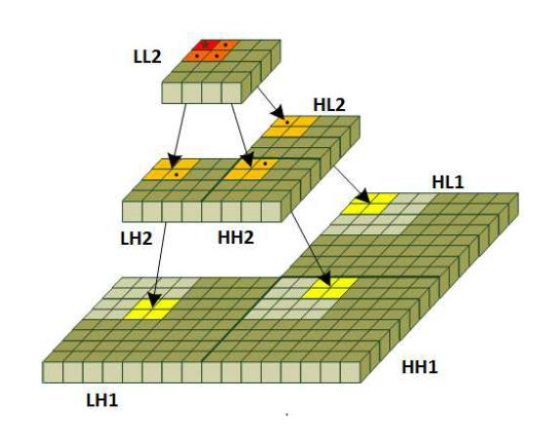
\includegraphics[width=0.5\textwidth]{lez7-WMSN/differentBitstreamsVideoVMSN.png}
		\caption{Trasmissione video su una WMSN con differenti bitstreams (codec FS-SPIHT)}
		\label{fig:WMSN-trasmissioneBitstreams}
	\end{figure}
